\section{Constraints on proton and nuclear structure}
\label{sec:protonPDFs}

By means of the strategy outlined in Sect.~\ref{sec:dis_pseudodata}, here
we quantify the impact on the proton PDFs
of differential  DIS
cross-section measurements exploiting the  LHC
neutrino beam. 
%
We assume an isoscalar free-nucleon target and neglect non-isoscalarity effects and nuclear modifications,
which are instead considered in Sect.~\ref{sec:nuclearPDFs}.
%
We present results first for the Hessian profiling of the PDF4LHC21,
and second for the Monte Carlo fit NNPDF4.0.
%
We study the stability of the results with respect to the inclusion of systematic uncertainties,
charm-tagged data, and lepton-charge separation.
%
We compare the impact of the different FPF experiments separately and also provide
results for their combination.

\subsection{Proton PDFs: impact on PDF4LHC21}
\label{sec:pdf4lhc21}

We begin by presenting results for the Hessian profiling of
the PDF4LHC21 NNLO set.
%
This proton PDF set is a Monte Carlo combination~\cite{Watt:2012tq,Carrazza:2015hva} of three global PDF sets, CT18~\cite{Hou:2019efy},
MSHT20~\cite{Bailey:2020ooq}, and NNPDF3.1~\cite{NNPDF:2017mvq}.
%
Its Hessian representations are obtained by means of the reduction methodologies developed in~\cite{Gao:2013bia,Carrazza:2015aoa}.
%
Being based on the combination of three modern global PDF fits, PDF4LHC21 provides a robust estimate
of  current uncertainties associated to our understanding of proton PDFs.
%
We profile PDF4LHC21 with pseudodata from various LHC neutrino experiments,
and study the stability of the results with respect to variations in the data
and methodology inputs.

Fig.~\ref{fig:FASERnu2_baseline} shows the
fractional uncertainties (at the 68\% confidence level) at $Q^2 = 10^4 \, \textrm{GeV}^2$ 
for the up and down valence quarks, gluon, total quark singlet, and total strangeness PDFs
in the PDF4LHC21 baseline, compared to the results obtained once the FASER$\nu$2 pseudo-data is added
by means of Hessian profiling.
%
The FASER$\nu$2 pseudo-data accounts for  both  inclusive and charm-tagged structure functions
and assumes outgoing lepton- charge identification.
%
We display results for the profiling in which the experimental covariance matrix
considers only statistical uncertainties, as well as for the scenario where
statistical and systematic errors are added in quadrature following
the procedure spelled out in Sect.~\ref{subsec:uncertainties}.
%
Note that in addition of a reduction of PDF uncertainties, the Hessian profiling
also results in general in a shift in the PDF central values.
%
This shift is however arbitrary since it 
depends on the fluctuations
entering the pseudo-data generation, and is hence ignored in the following.

%%%%%%%%%%%%%%%%%%%%%%%%%%%%%%%%%%%%%%%%%%%%%%%%%%%%%%%%%%%%%%%%%%%%%%%%
\begin{figure}[t]
\centering
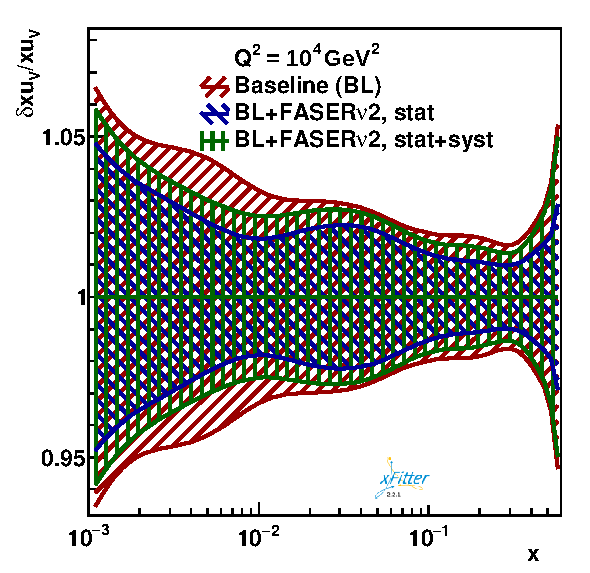
\includegraphics[width=0.32\textwidth]{plots/proton_fasernu2/inclusive+charm_chargediscrimination/fred05fcorr05_FASERv2_q2_10000_pdf_uv_ratio.pdf}
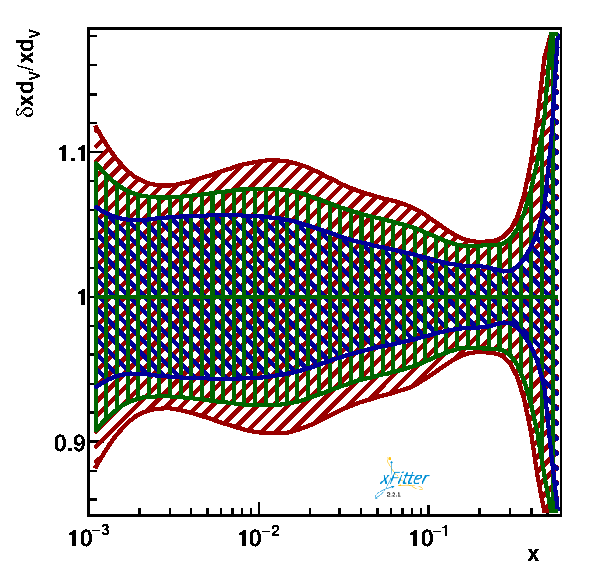
\includegraphics[width=0.32\textwidth]{plots/proton_fasernu2/inclusive+charm_chargediscrimination/fred05fcorr05_FASERv2_q2_10000_pdf_dv_ratio.pdf}
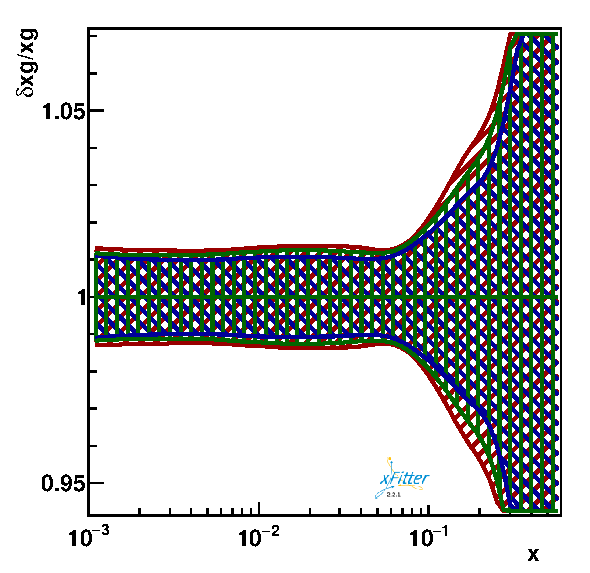
\includegraphics[width=0.32\textwidth]{plots/proton_fasernu2/inclusive+charm_chargediscrimination/fred05fcorr05_FASERv2_q2_10000_pdf_g_ratio.pdf}\\
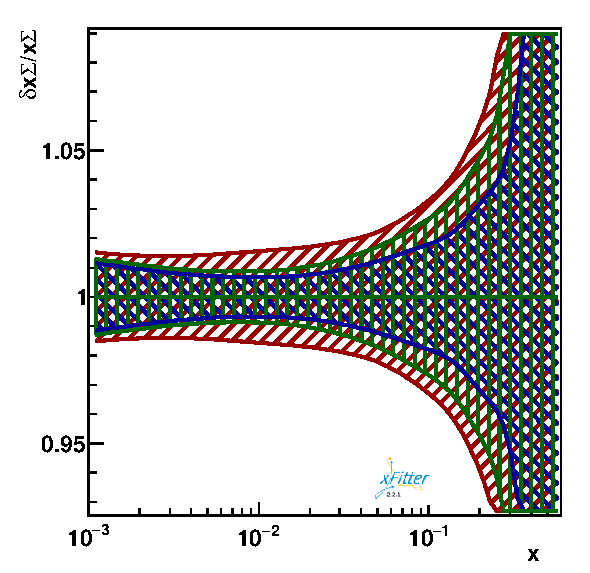
\includegraphics[width=0.32\textwidth]{plots/proton_fasernu2/inclusive+charm_chargediscrimination/fred05fcorr05_FASERv2_q2_10000_pdf_Sea_ratio.pdf}
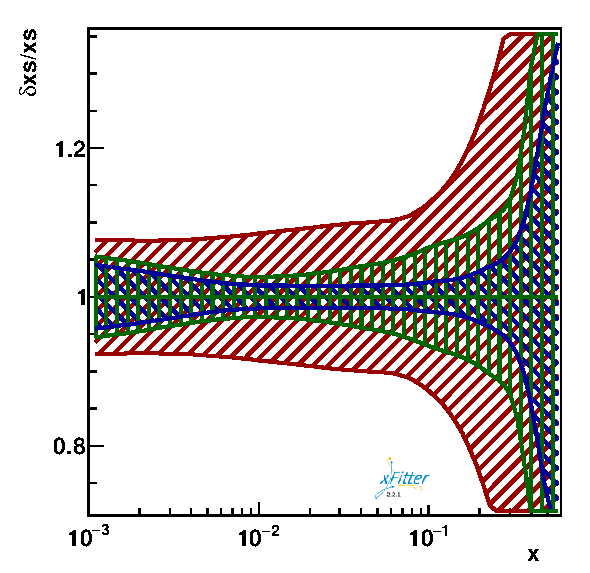
\includegraphics[width=0.32\textwidth]{plots/proton_fasernu2/inclusive+charm_chargediscrimination/fred05fcorr05_FASERv2_q2_10000_pdf_s_ratio.pdf}
\caption{
The fractional uncertainties (68\% confidence level) at $Q^2 = 10^4 \, \textrm{GeV}^2$ 
for the up and down valence quarks, gluon, total quark singlet, and total strangeness PDFs
in the PDF4LHC21 baseline, compared to the results obtained once the FASER$\nu$2 pseudo-data is included.
%
The FASER$\nu$2 impact projections are provided both without and with systematic
uncertainties accounted for.
%
We include  both  inclusive and charm-tagged structure functions
and assume outgoing lepton charge-separation.
%
}
\label{fig:FASERnu2_baseline}
\end{figure}
%%%%%%%%%%%%%%%%%%%%%%%%%%%%%%%%%%%%%%%%%%%%%%%%%%%%%%%%%%%%%%%%%%%%%%%%

Inspection of Fig.~\ref{fig:FASERnu2_baseline} reveals that measurement of DIS structure
functions at FASER$\nu$2 impose stringent constraints on the quark PDFs, while leaving
the gluon PDF essentially unaffected.
%
As expected for a neutrino scattering experiment, its impact is most marked for
those PDF combinations sensitive to quark flavour separation such as $u_V$, $d_V$, and
$s^+$.
%
The reduction of PDF uncertainties is particularly significant for the total strangeness PDF,
as  consequence of the inclusion of charm-tagged structure functions in the fit as we demonstrate below.
%
Crucially, one finds that for the assumptions on the systematic uncertainties
discussed in Sect~\ref{sec:dis_pseudodata}, the PDF sensitivity is only marginally degraded
as compared to the case in which systematic errors are neglected.
%
This result is consistent with Fig.~\ref{fig:percentage_uncertainties_overview}, showing
how in most bins systematic and statistical errors are of similar magnitude.

In the following, we consider the results obtained using only statistical uncertainties as the baseline, 
and examine stability of these results with respect to the chosen experiment and integrated luminosity, the modelling of systematic
uncertainties, being able to identify or not charm production, and being able to tell part outgoing
charged leptons from anti-leptons.


%
Fig.~\ref{fig:profiling_charm} displays a comparison of the baseline LHC neutrino dataset with the results
of profiling without the charm production structure functions. 
Particularly, the constraints on the $s$ PDF are observed to become more stringent 
by virtue of the contribution of the charm production structure functions.

%%%%%%%%%%%%%%%%%%%%%%%%%%%%%%%%%%%%%%%%%%%%%%%%%%%%%%%%%%%%%%%%%%%%%%%%
\begin{figure}[t]
\centering
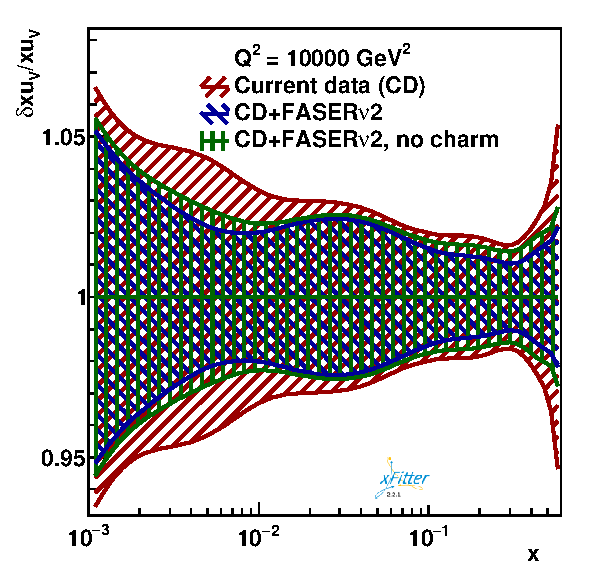
\includegraphics[width=0.32\textwidth]{plots/proton_fasernu2/inclusive-only_vs_inclusive+charm/statOnly_FASERv2_q2_10000_pdf_uv_ratio.pdf}
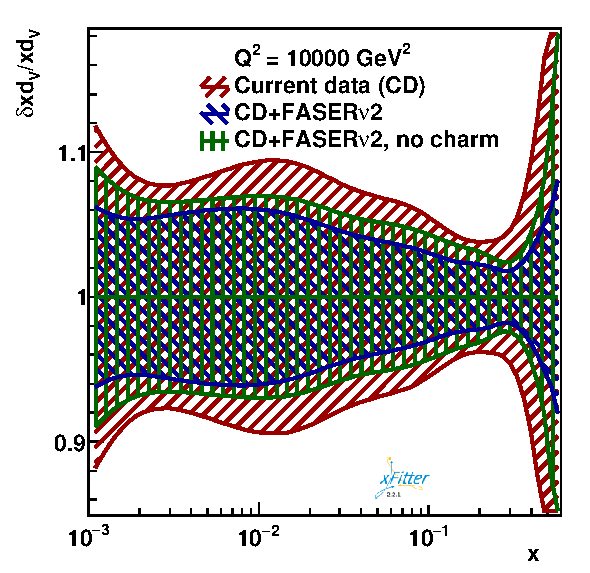
\includegraphics[width=0.32\textwidth]{plots/proton_fasernu2/inclusive-only_vs_inclusive+charm/statOnly_FASERv2_q2_10000_pdf_dv_ratio.pdf}
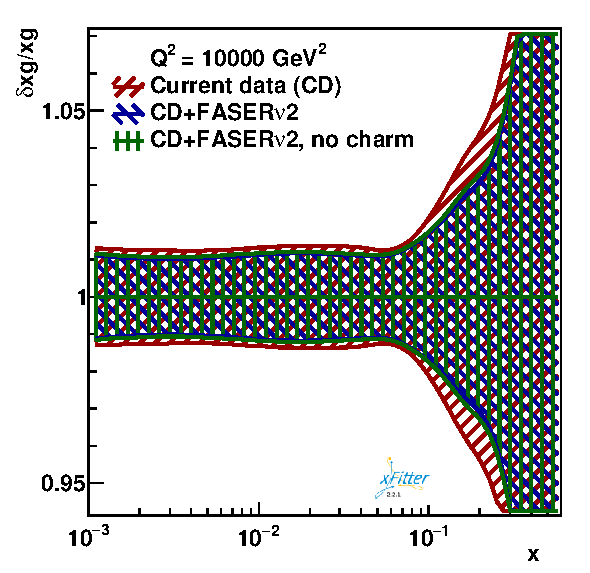
\includegraphics[width=0.32\textwidth]{plots/proton_fasernu2/inclusive-only_vs_inclusive+charm/statOnly_FASERv2_q2_10000_pdf_g_ratio.pdf}\\
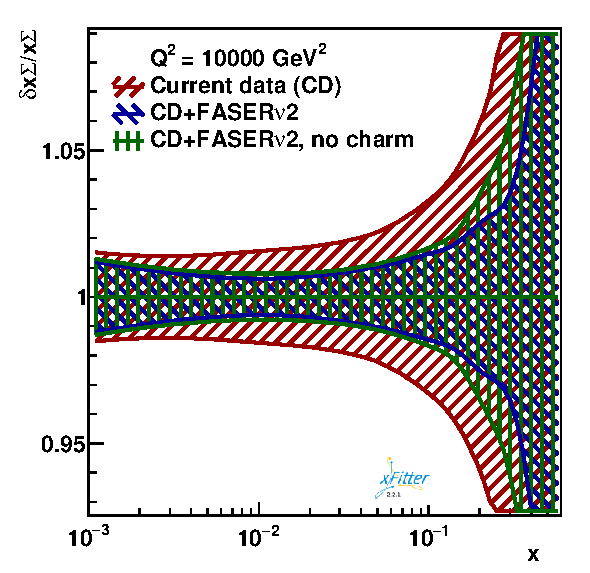
\includegraphics[width=0.32\textwidth]{plots/proton_fasernu2/inclusive-only_vs_inclusive+charm/statOnly_FASERv2_q2_10000_pdf_Sea_ratio.pdf}
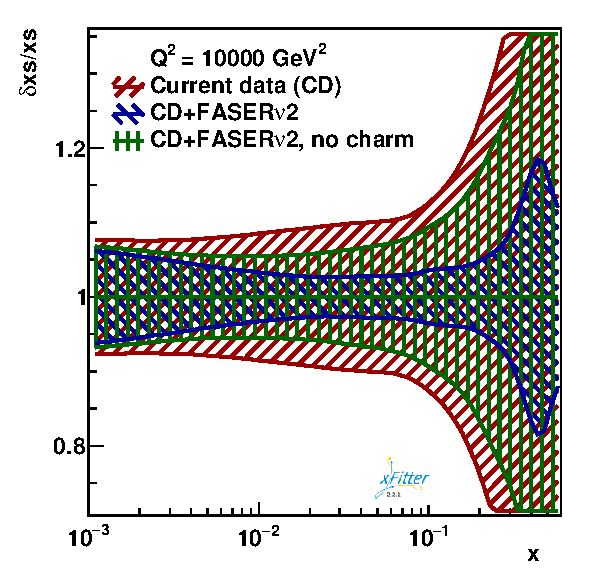
\includegraphics[width=0.32\textwidth]{plots/proton_fasernu2/inclusive-only_vs_inclusive+charm/statOnly_FASERv2_q2_10000_pdf_s_ratio.pdf}
\caption{Same as Fig.~\ref{fig:FASERnu2_baseline} (statistical uncertainties only),
  now showing results in the scenario where charm-tagged structure function measurements
  are excluded from the analysis.
}
\label{fig:FASERnu2_nocharm}
\end{figure}
%%%%%%%%%%%%%%%%%%%%%%%%%%%%%%%%%%%%%%%%%%%%%%%%%%%%%%%%%%%%%%%%%%%%%%%%

%
Fig.~\ref{fig:profiling_nochargediscrimination} compares the baseline LHC neutrino dataset with the results
of a profiling without allowing for the possibility of outgoing lepton charge separation.


%%%%%%%%%%%%%%%%%%%%%%%%%%%%%%%%%%%%%%%%%%%%%%%%%%%%%%%%%%%%%%%%%%%%%%%%
\begin{figure}[t]
\centering
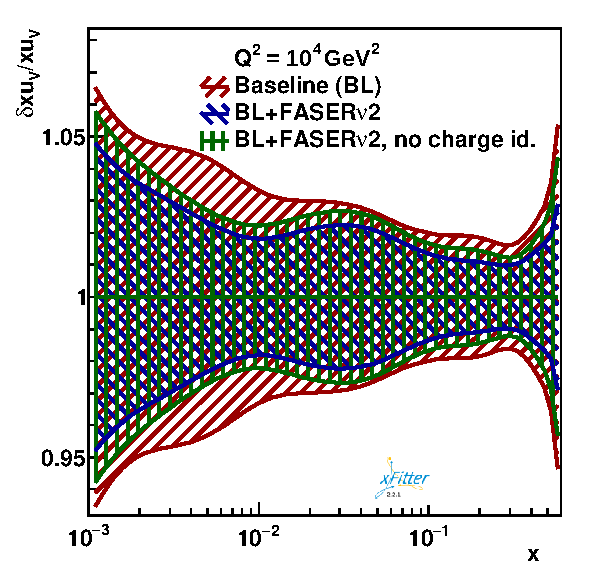
\includegraphics[width=0.32\textwidth]{plots/proton_fasernu2/nochargediscrimination/statOnly_FASERv2_q2_10000_pdf_uv_ratio.pdf}
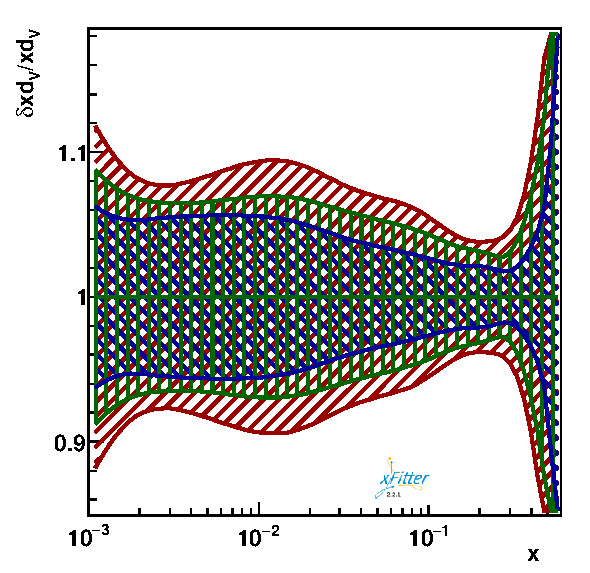
\includegraphics[width=0.32\textwidth]{plots/proton_fasernu2/nochargediscrimination/statOnly_FASERv2_q2_10000_pdf_dv_ratio.pdf}
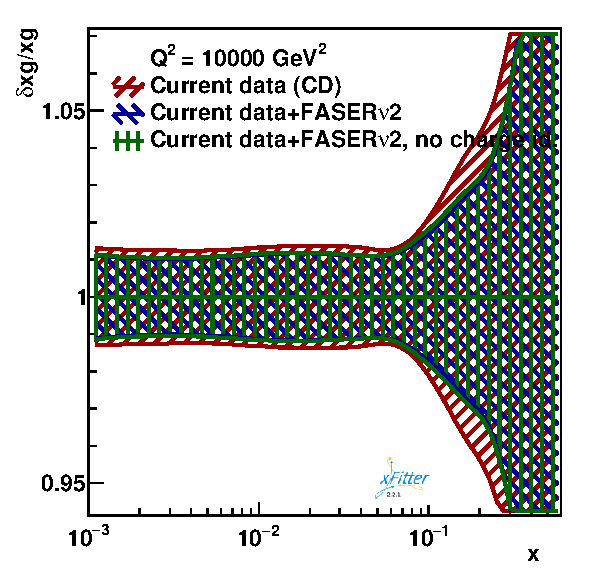
\includegraphics[width=0.32\textwidth]{plots/proton_fasernu2/nochargediscrimination/statOnly_FASERv2_q2_10000_pdf_g_ratio.pdf}\\
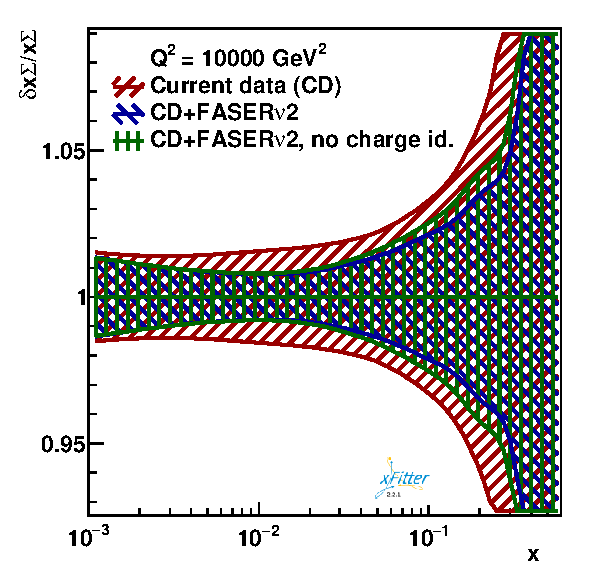
\includegraphics[width=0.32\textwidth]{plots/proton_fasernu2/nochargediscrimination/statOnly_FASERv2_q2_10000_pdf_Sea_ratio.pdf}
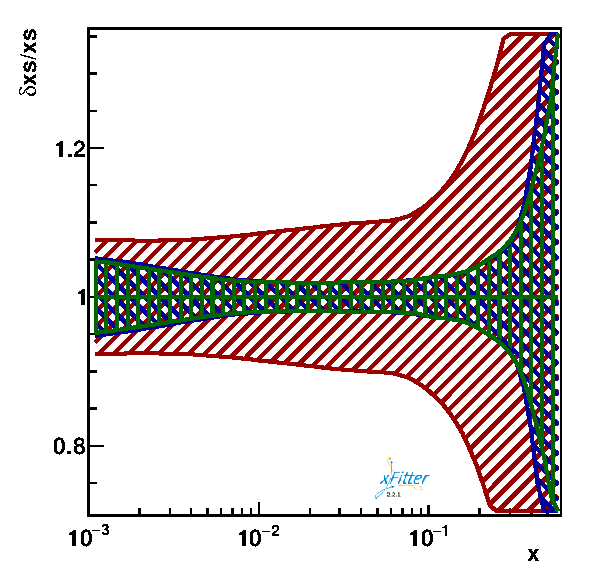
\includegraphics[width=0.32\textwidth]{plots/proton_fasernu2/nochargediscrimination/statOnly_FASERv2_q2_10000_pdf_s_ratio.pdf}
\caption{Same as Fig.~\ref{fig:FASERnu2_baseline} (statistical uncertainties only),
  now showing results in the scenario where the charge of the final-state charged lepton
  cannot be identified.
 }
\label{fig:FASERnu2_nochargeID}
\end{figure}
%%%%%%%%%%%%%%%%%%%%%%%%%%%%%%%%%%%%%%%%%%%%%%%%%%%%%%%%%%%%%%%%%%%%%%%%



Besides FASER$u$2, further FPF detectors may also be used for constraining the PDFs. 
Fig.~\ref{fig:profiling_FASERv2_vs_AdvSND} illustrates the effect of using the AdvSND pseudodata alone, 
shown together with the previous result of using only FASER$\nu$2 pseudodata. 
Fig.~\ref{fig:profiling_FASERv2_vs_FLArE10} shows a similar comparison, 
but using FLArE pseudodata instead of AdvSND. 
Most importantly however, all these datasets can be included to obtain a complete FPF result, 
shown in Fig.~\ref{fig:profiling_FPF}.

%%%%%%%%%%%%%%%%%%%%%%%%%%%%%%%%%%%%%%%%%%%%%%%%%%%%%%%%%%%%%%%%%%%%%%%%
\begin{figure}[t]
\centering
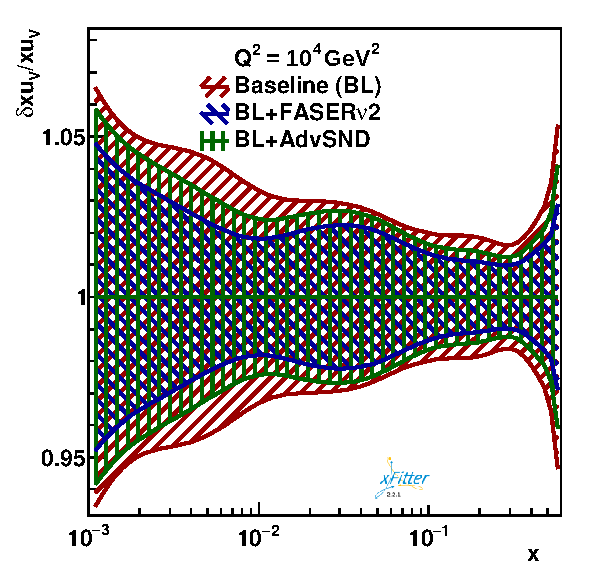
\includegraphics[width=0.32\textwidth]{plots/proton_fasernu2/FASERv2_vs_AdvSND/statOnly_AdvSND_q2_10000_pdf_uv_ratio.pdf}
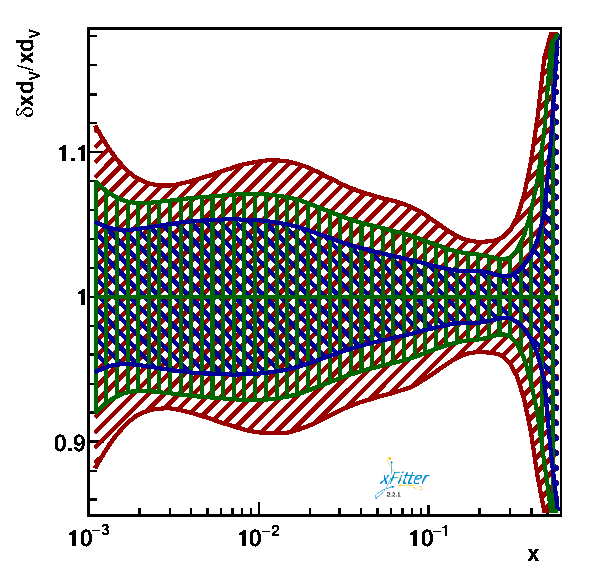
\includegraphics[width=0.32\textwidth]{plots/proton_fasernu2/FASERv2_vs_AdvSND/statOnly_AdvSND_q2_10000_pdf_dv_ratio.pdf}
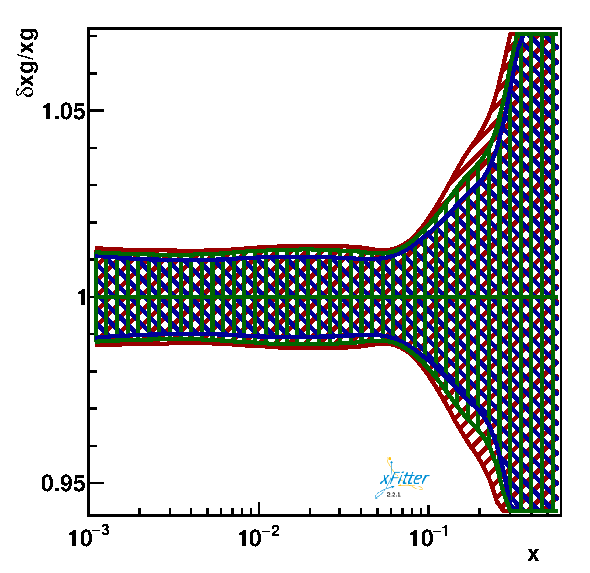
\includegraphics[width=0.32\textwidth]{plots/proton_fasernu2/FASERv2_vs_AdvSND/statOnly_AdvSND_q2_10000_pdf_g_ratio.pdf}\\
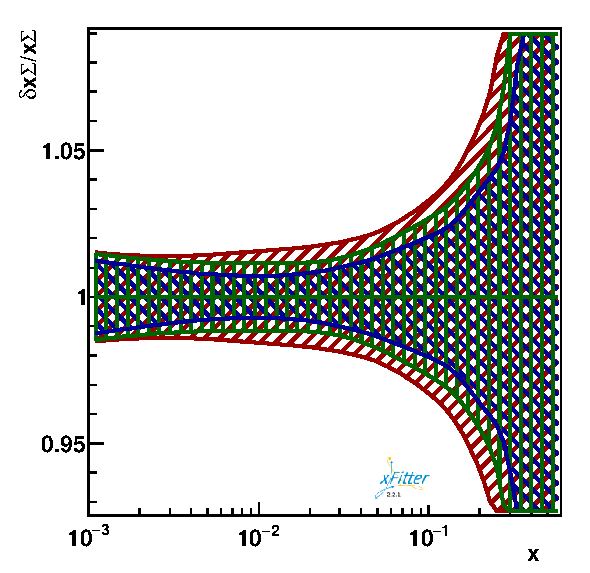
\includegraphics[width=0.32\textwidth]{plots/proton_fasernu2/FASERv2_vs_AdvSND/statOnly_AdvSND_q2_10000_pdf_Sea_ratio.pdf}
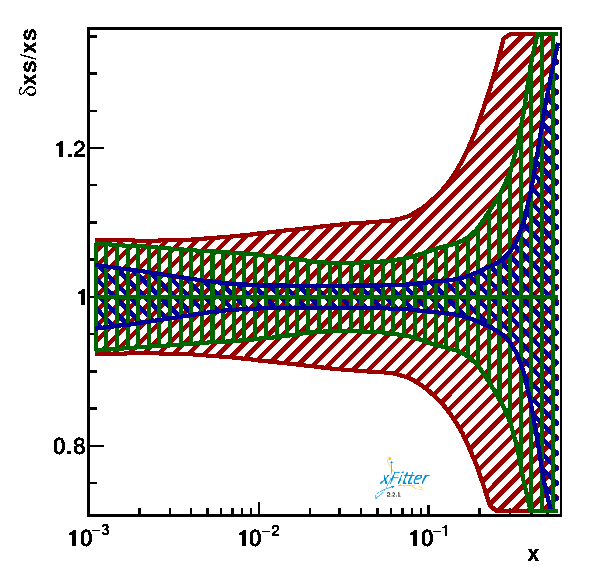
\includegraphics[width=0.32\textwidth]{plots/proton_fasernu2/FASERv2_vs_AdvSND/statOnly_AdvSND_q2_10000_pdf_s_ratio.pdf}
\caption{
  Same as  Fig.~\ref{fig:FASERnu2_baseline} (statistical uncertainties only), comparing
  the projected PDF impact of FASER$\nu$2 with that of AdvSND.
}
\label{fig:FASERnu2_advsnd}
\end{figure}
%%%%%%%%%%%%%%%%%%%%%%%%%%%%%%%%%%%%%%%%%%%%%%%%%%%%%%%%%%%%%%%%%%%%%%%%

%%%%%%%%%%%%%%%%%%%%%%%%%%%%%%%%%%%%%%%%%%%%%%%%%%%%%%%%%%%%%%%%%%%%%%%%%%%%%
\begin{figure}[t]
\centering
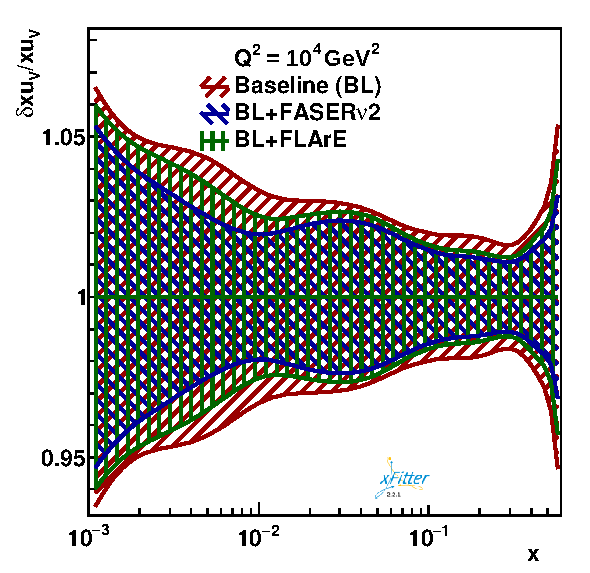
\includegraphics[width=0.32\textwidth]{plots/proton_fasernu2/FASERv2_vs_FLArE10/statOnly_FLArE10_q2_10000_pdf_uv_ratio.pdf}
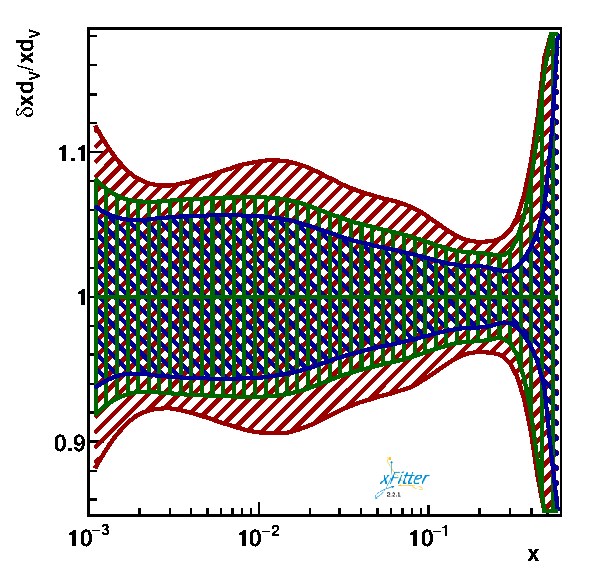
\includegraphics[width=0.32\textwidth]{plots/proton_fasernu2/FASERv2_vs_FLArE10/statOnly_FLArE10_q2_10000_pdf_dv_ratio.pdf}
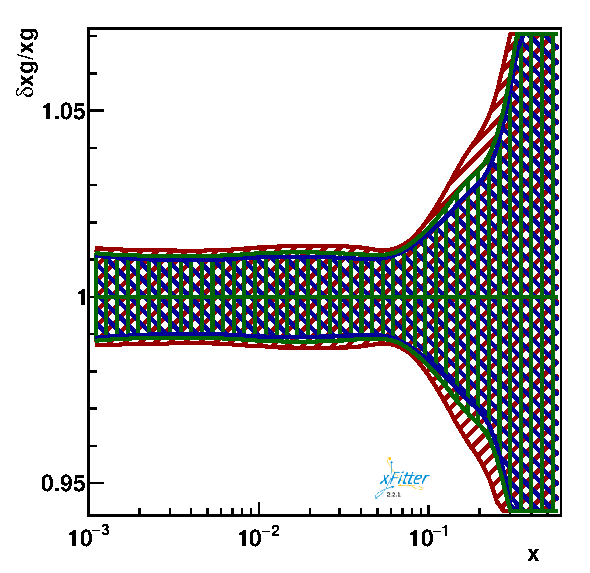
\includegraphics[width=0.32\textwidth]{plots/proton_fasernu2/FASERv2_vs_FLArE10/statOnly_FLArE10_q2_10000_pdf_g_ratio.pdf}\\
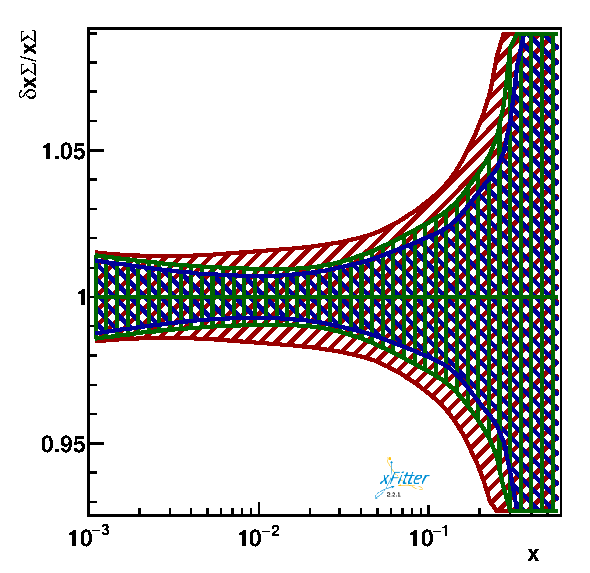
\includegraphics[width=0.32\textwidth]{plots/proton_fasernu2/FASERv2_vs_FLArE10/statOnly_FLArE10_q2_10000_pdf_Sea_ratio.pdf}
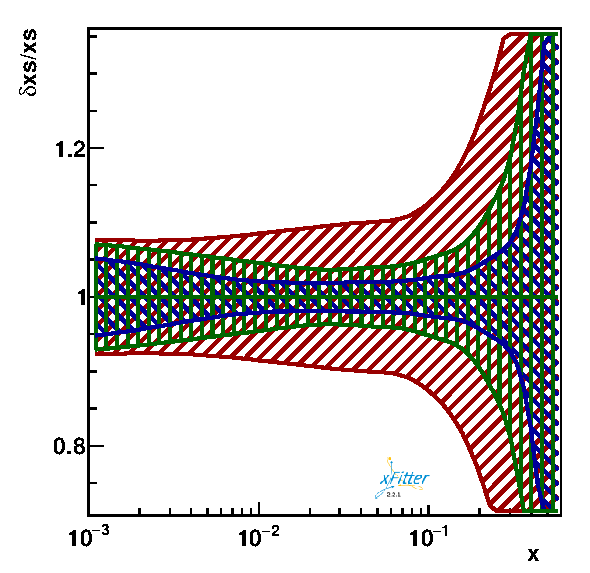
\includegraphics[width=0.32\textwidth]{plots/proton_fasernu2/FASERv2_vs_FLArE10/statOnly_FLArE10_q2_10000_pdf_s_ratio.pdf}
\caption{
  Same as Fig.~\ref{fig:FASERnu2_advsnd},
  comparing
  the projected PDF impact of FASER$\nu$2 with that of FLArE10. 
}
\label{fig:FASERnu2_FLAre10}
\end{figure}
%%%%%%%%%%%%%%%%%%%%%%%%%%%%%%%%%%%%%%%%%%%%%%%%%%%%%%%%%%%%%%%%%%%%%%

%%%%%%%%%%%%%%%%%%%%%%%%%%%%%%%%%%%%%%%%%%%%%%%%%%%%%%%%%%%%%%%%%%%%%%%
\begin{figure}[t]
\centering
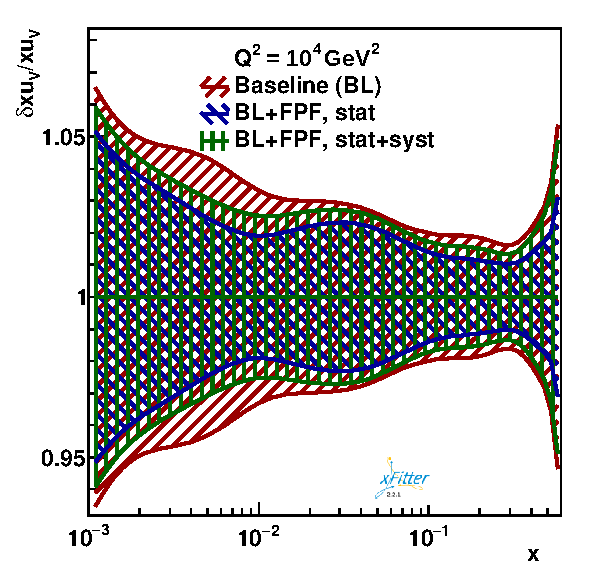
\includegraphics[width=0.32\textwidth]{plots/proton_fasernu2/FPF/fred05fcorr05_FPF_q2_10000_pdf_uv_ratio.pdf}
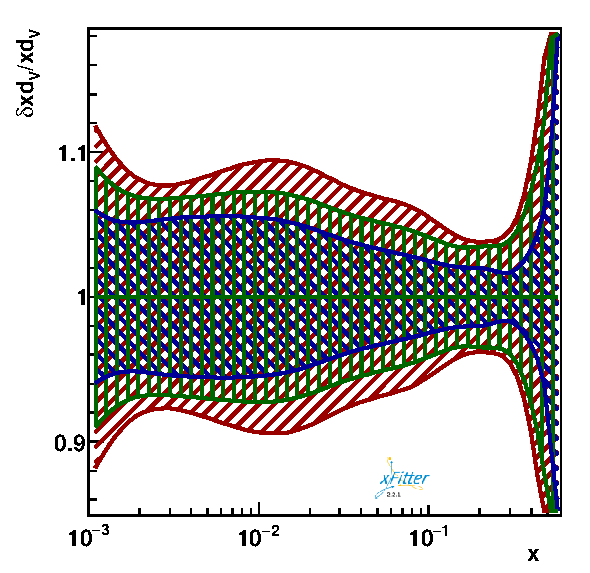
\includegraphics[width=0.32\textwidth]{plots/proton_fasernu2/FPF/fred05fcorr05_FPF_q2_10000_pdf_dv_ratio.pdf}
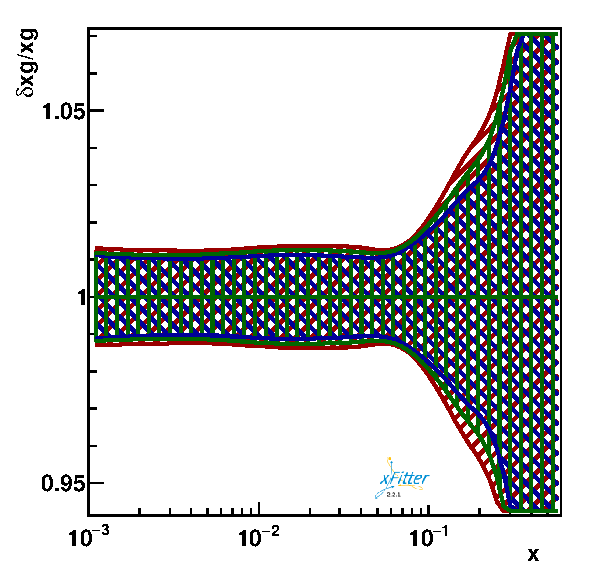
\includegraphics[width=0.32\textwidth]{plots/proton_fasernu2/FPF/fred05fcorr05_FPF_q2_10000_pdf_g_ratio.pdf}\\
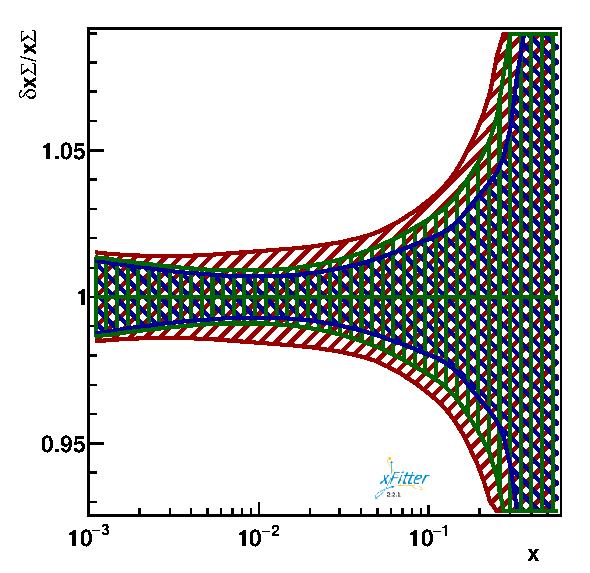
\includegraphics[width=0.32\textwidth]{plots/proton_fasernu2/FPF/fred05fcorr05_FPF_q2_10000_pdf_Sea_ratio.pdf}
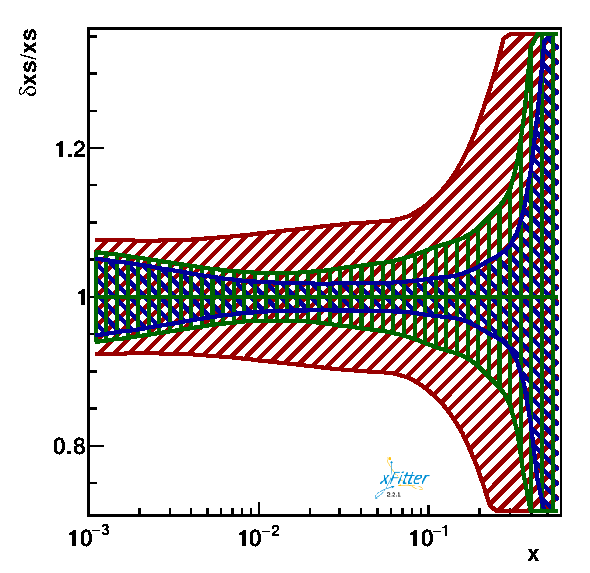
\includegraphics[width=0.32\textwidth]{plots/proton_fasernu2/FPF/fred05fcorr05_FPF_q2_10000_pdf_s_ratio.pdf}
\caption{
  Same as Fig.~\ref{fig:FASERnu2_baseline} now quantifying the
  projected PDF impact of the three FPF experiments added simultaneously to
  the analysis: FASER$\nu$2, AdvSND, and FLArE10. 
}
\label{fig:profiling_FPF}
\end{figure}
%%%%%%%%%%%%%%%%%%%%%%%%%%%%%%%%%%%%%%%%%%%%%%%%%%%%%%%%%%%%%%%%%%%%%%%

\clearpage


\subsection{Proton PDFs: impact on NNPDF4.0}
\label{sec:nnpdf40}

Selection of the {\sc\small xFitter} results for the NNPDF case.

Fig.~\ref{fig:nnpdf40_fasernu2_baseline} presents the same comparison
as in Fig.~\ref{fig:profiling_syst} now for
 the fits
 based on the NNPDF4.0 global analysis.
 %
 The impact on the PDFs found by direct inclusion of the FPF structure
 functions on the NNPDF4.0 fit is qualitatively consistent with
 that found from the Hessian profiling of PDF4LHC21.

%%%%%%%%%%%%%%%%%%%%%%%%%%%%%%%%%%%%%%%%%%%%%%%%%%%%%%%%%%%%%%%%%%%%%%%%
\begin{figure}[t]
\centering
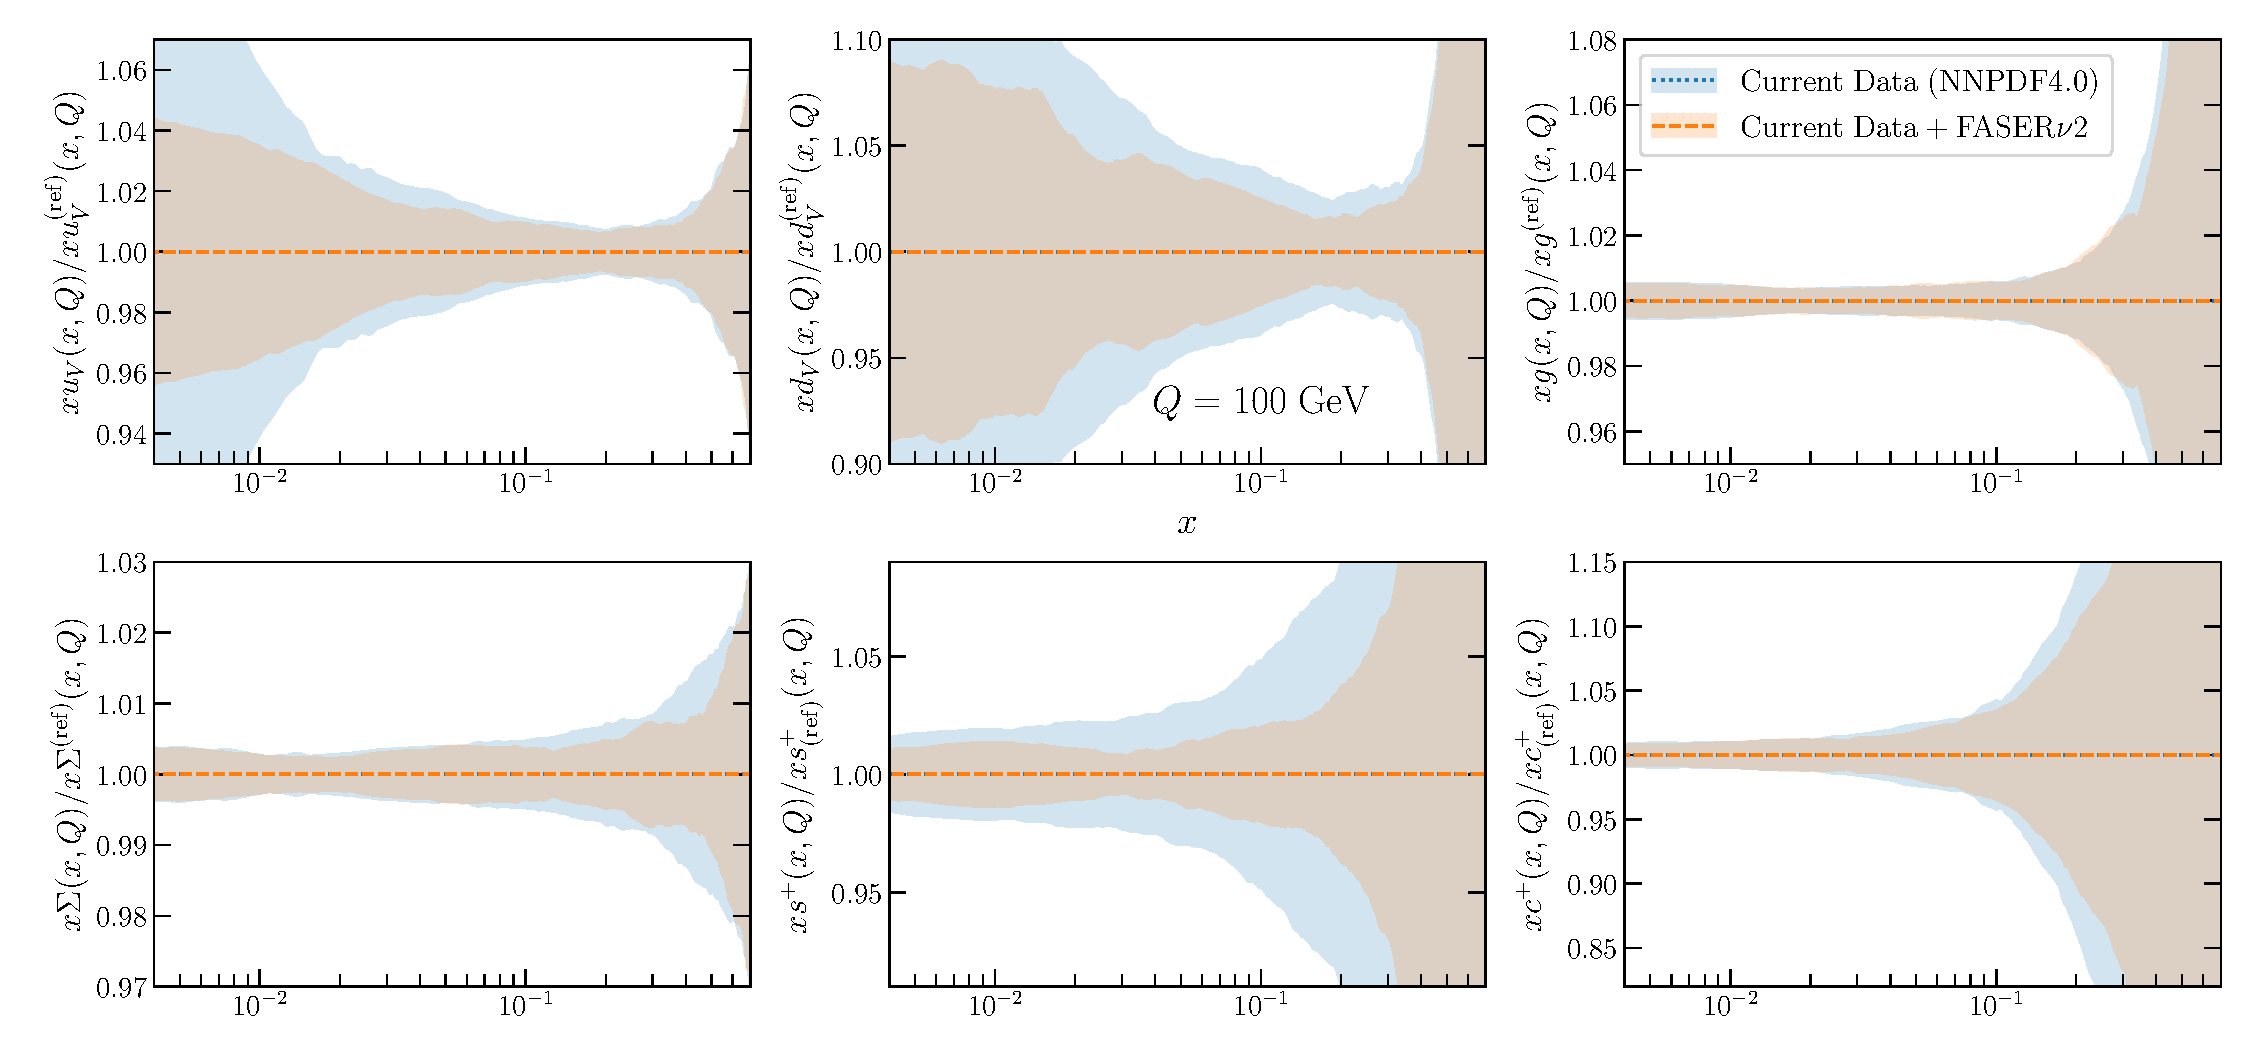
\includegraphics[width=0.99\textwidth]{plots/FASERnu2-q100gev-ratios.pdf}
\caption{
  Same as Fig.~\ref{fig:profiling_syst} now for the fits
  based on the NNPDF4.0 global analysis.
%
}
\label{fig:nnpdf40_fasernu2_baseline}
\end{figure}
%%%%%%%%%%%%%%%%%%%%%%%%%%%%%%%%%%%%%%%%%%%%%%%%%%%%%%%%%%%%%%%%%%%%%%%%

\clearpage

\subsection{Nuclear PDFs: impact on EPPS21}
\label{sec:nuclearPDFs}

The study presented in Sect.~\ref{sec:protonPDFs} treated, from the point of view
of PDF constraints, the neutrino scattering target
as composed by isoscalar free-nucleons, and hence neglecting nuclear modifications
and non-isoscalar effects.
%
We now revisit this analysis but accounting for the fact that the target materials in the FPF
experiments actually
composed by heavy nuclei, specifically by tungsten (the exception is FLArE with liquid argon, which
is however not considered here).
%
Nuclear modifications associated to a tungsten target are not necessarily small as compared
to a free isoscalar nucleon, and hence will affect the event rate predictions for
the FPF experiments.
%
Turning the argument around, measurements of differential neutrino cross-sections
on heavy nuclear targets provide direct constraints on these nuclear modifications
without replying on assumptions on the $A$ dependence.

For this exercise, the prior nuclear PDF set is taken to be EPPS21, a global determination
that accounts for the constraints of existing datasets involving nuclei as target or projectiles.
%
In particular, EPPS21 already includes information from neutrino DIS on nuclear targets
from the CHORUS and NuTeV experiments.
%
The application of Hessian profiling to EPPS21 follows the same strategy as that
for PDF4LHC21, with the caveat that its Hessian error sets also include the contribution
from the uncertainties  associated to their reference proton PDF set, in this case CT18.
%
Given that the measured event rates depend on both the proton PDFs and the nuclear modifications,
when profiling EPPS21 we also account for the Hessian sets associated to the CT18 proton
PDF dependence.

Fig.~\ref{fig:profiling_syst_nuclear} displays the baseline result of the profiling using the EPPS21 global determination of nuclear PDFs,
specifically of the set with $A=184$ (tungsten target).
%
Also in this case we consider first the impact of the baseline LHC neutrino dataset, consisting
on the FASER$\nu$2 experiment inclusive and charm structure functions,  and charge flavour
separation. 
The bands indicate the 68\% CL uncertainties, 
both for the case assuming statistical uncertainties only, 
as well as including an estimate for both statistical and systematic uncertainties.
The result from using the full FPF set comprising of AdvSND, FASER$\nu$2 and FLArE pseudodata is shown in Fig.~\ref{fig:profiling_FPF_nuclear}.

%%%%%%%%%%%%%%%%%%%%%%%%%%%%%%%%%%%%%%%%%%%%%%%%%%%%%%%%%%%%%%%%%%%%%%%%
\begin{figure}[t]
\centering
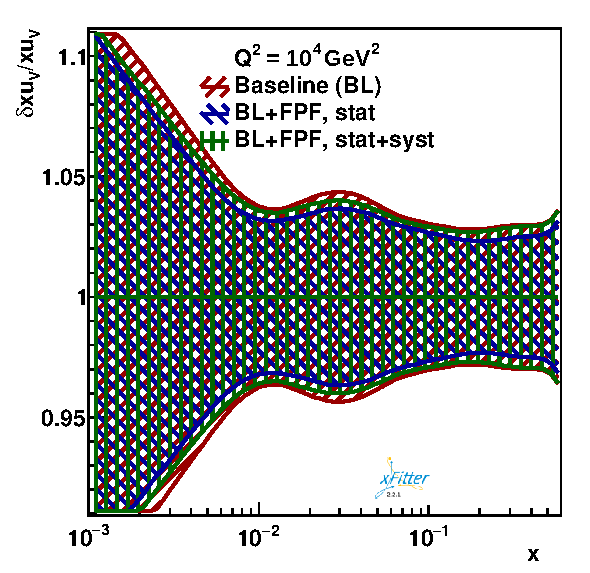
\includegraphics[width=0.32\textwidth]{plots/nuclear_fasernu2/FPF/fred05fcorr05_FPF_q2_10000_pdf_uv_ratio.pdf}
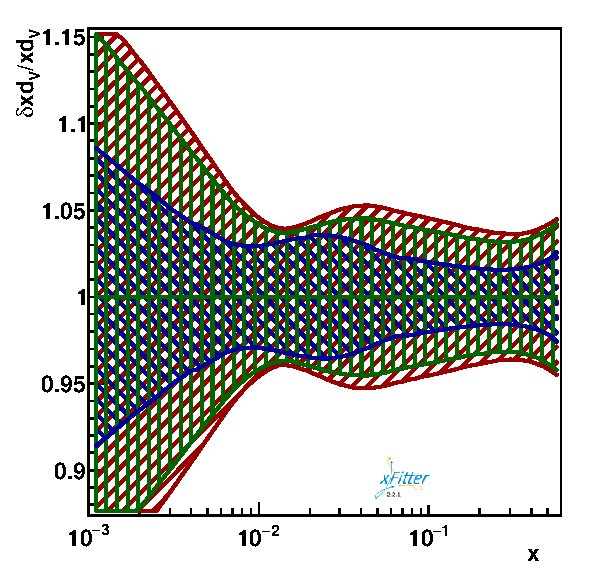
\includegraphics[width=0.32\textwidth]{plots/nuclear_fasernu2/FPF/fred05fcorr05_FPF_q2_10000_pdf_dv_ratio.pdf}
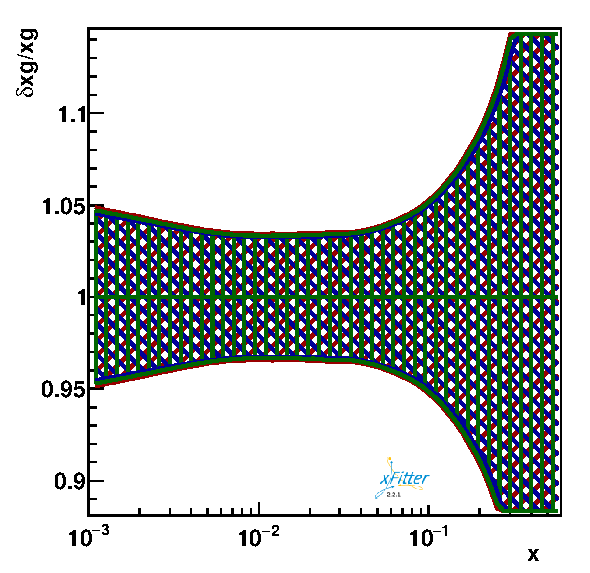
\includegraphics[width=0.32\textwidth]{plots/nuclear_fasernu2/FPF/fred05fcorr05_FPF_q2_10000_pdf_g_ratio.pdf}\\
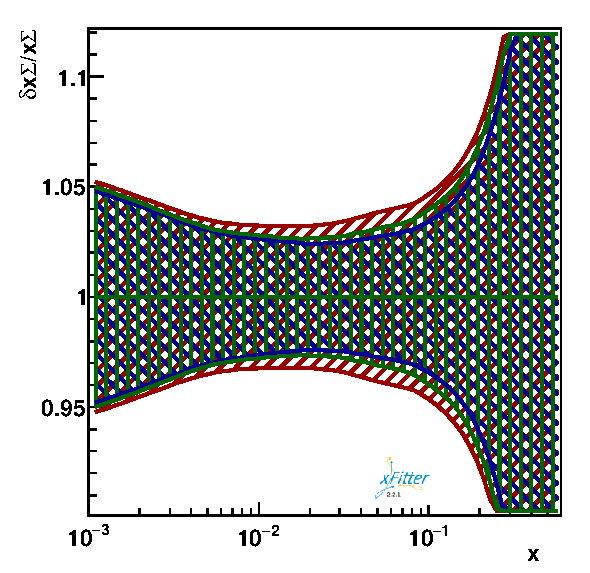
\includegraphics[width=0.32\textwidth]{plots/nuclear_fasernu2/FPF/fred05fcorr05_FPF_q2_10000_pdf_Sea_ratio.pdf}
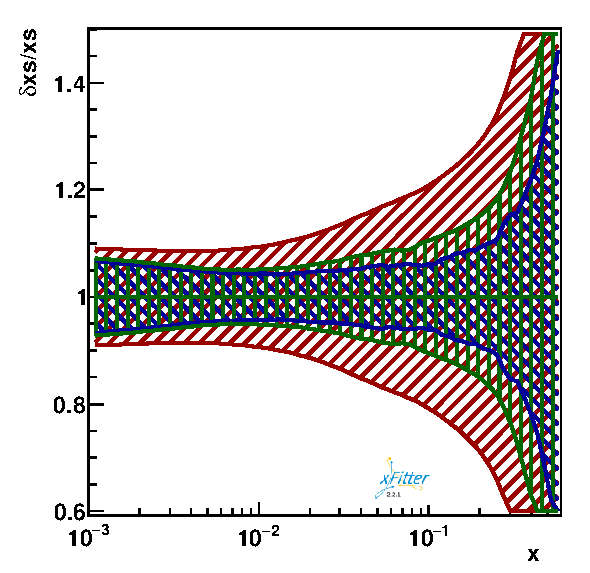
\includegraphics[width=0.32\textwidth]{plots/nuclear_fasernu2/FPF/fred05fcorr05_FPF_q2_10000_pdf_s_ratio.pdf}
\caption{The impact of the full FPF pseudodataset in profiling using the EPPS21 global determination of nuclear PDFs (red), specifically for $A=184$. The 68\% CL uncertainty bands resulting from assuming only statistical (statistical and systematic) uncertainties are shown in blue (green).
}
\label{fig:profiling_FPF_nuclear}
\end{figure}
%%%%%%%%%%%%%%%%%%%%%%%%%%%%%%%%%%%%%%%%%%%%%%%%%%%%%%%%%%%%%%%%%%%%%%%%
